\documentclass[english, 11pt]{article}
\usepackage{graphicx}
\usepackage{amsmath}
\usepackage{hyperref}
\usepackage{setspace}
\usepackage{apacite}
\usepackage{hyperref}
\usepackage[sort]{natbib}
\usepackage{pxfonts}
\usepackage[utf8]{inputenc}
\usepackage[left=1in,right=1in,top=1in,bottom=1in]{geometry}
\usepackage[left]{lineno}
\usepackage{soul}
\linenumbers

\newcommand{\varExplained}{S1}
\newcommand{\topTerms}{S2}
\newcommand{\componentBrains}{S3}
\newcommand{\topicContrasts}{S4}
\newcommand{\neurosynthFull}{S5}

\newcommand{\topics}{S1}
\newcommand{\topicTags}{S2}

\title{High-level cognition is supported by information-rich but compressible brain activity patterns}

\author{Lucy L. W. Owen\textsuperscript{1, 2} and Jeremy R. Manning\textsuperscript{1,
*}\\\textsuperscript{1}Department of Psychological and Brain Sciences,\\Dartmouth College,
Hanover, NH\\[0.1cm]\textsuperscript{2}Carney Institute for Brain Sciences,\\Brown University,
Providence, RI\\[0.1cm] \textsuperscript{*}Address correspondence to
jeremy.r.manning@dartmouth.edu}

\begin{document}
\maketitle


\begin{abstract} 

We applied dimensionality reduction algorithms and pattern classifiers to
functional neuroimaging data collected as participants listened to a story,
temporally scrambled versions of the story, or underwent a resting state
scanning session. These experimental conditions were intended to require
different depths of processing and inspire different levels of cognitive
engagement. We considered two primary aspects of the data. First, we treated
the maximum achievable decoding accuracy across participants as an indicator of
the ``informativeness'' of the recorded patterns. Second, we treated the number
of features (components) required to achieve a threshold decoding accuracy as a
proxy for the ``compressibility'' of the neural patterns (where fewer
components indicate greater compression). Overall, we found that the peak
decoding accuracy (achievable without restricting the numbers of features)
was highest in the intact (unscrambled) story listening condition.  However, the
number of features required to achieve comparable classification accuracy
was also lowest in the intact story listening condition.  Taken together, our work
suggests that our brain networks flexibly reconfigure according to ongoing task
demands, and that the activity patterns associated with higher-order cognition
and high engagement are both more informative and more compressible than the
activity patterns associated with lower-order tasks and lower levels of
engagement.

\bigskip
\noindent
\textbf{Keywords: information, compression, temporal decoding, dimensionality
reduction, neuroimaging}

\end{abstract}

\doublespacing

\section*{Introduction}

Large-scale networks, including the human brain, may be conceptualized as
occupying one or more positions along on a continuum. At one extreme, every
node is fully independent from every other node. At the other extreme, all
nodes behave identically. Each extreme optimizes key properties of how the
network functions. When every node is independent, the network is maximally
\textit{expressive}: if we define the network's ``state'' as the activity
pattern across its nodes, then every state is equally reachable by a network
with fully independent nodes. On the other hand, a network of identically
behaved nodes optimizes \textit{robustness}: any subset of nodes may be removed
from the network without any loss of function or expressive power, as long as
any single node remains. Presumably, most natural systems tend to occupy
positions between these extremes. We wondered: might the human brain
reconfigure itself to be more flexible or more robust according to ongoing
demands? In other words, might the brain reconfigure its connections or
behaviors under different circumstances to change its position along this
continuum?

Closely related to the above notions of expressiveness versus robustness are
measures of how much \textit{information} is contained in a given signal or
pattern, and how \textit{redundant} a signal is~\citep{Shan48}. Formally,
information is defined as the amount of uncertainty about a given variables'
outcomes (i.e., entropy), measured in \textit{bits}, or the optimal number of
yes/no questions needed to reduce uncertainty about the variable's outcomes to
zero. Highly complex systems with many degrees of freedom (i.e., high
flexibility and expressiveness), are more information-rich than simpler or more
constrained systems. The redundancy of a signal denotes the difference between
how expressive the signal \textit{could} be (i.e., proportional to the number
of unique states or symbols used to transmit the signal) and the actual
information rate (i.e., the entropy of each individual state or symbol). If a
brain network's nodes are fully independent, then the number of bits required
to express a single activity pattern is proportional to the number of nodes.
The network would also be minimally redundant, since the status of every node
would be needed to fully express a single brain activity pattern. If a brain
network's nodes are fully coupled and identical, then the number of bits
required to express a single activity pattern is proportional to the number of
unique states or values any individual node can take on. Such a network would
be highly redundant, since knowing any individual node's state would be
sufficient to recover the full-brain activity pattern. Highly redundant systems
are also robust, since there is little total information loss due to removing
any given observation.

We take as a given that brain activity is highly flexible: our brains can
exhibit nearly infinite varieties of activity patterns. This flexibility
implies that our brains' activity patterns are highly information rich. However,
brain activity patterns are also highly structured. For example, full-brain
correlation matrices are stable within~\citep{FinnEtal15, FinnEtal17,
GratEtal18} and across~\citep{YeoEtal11, GlerEtal12, GratEtal18, ColeEtal14}
individuals. This stability suggests that our brains' activity patterns are at
least partially constrained, for example by anatomical, external, or internal
factors. Constraints on brain activity that limit its flexibility decrease
expressiveness (i.e., its information rate). However, constraints on brain
activity also increase its robustness to noise (e.g., ``missing'' or corrupted
signals may be partially recovered). For example, recent work has shown that
full-brain activity patterns may be reliably recovered from only a relatively
small number of implanted electrodes~\citep{OwenEtal20, ScanEtal21}. This
robustness property suggests that the relevant signal (e.g., underlying factors
that have some influence over brain activity patterns) are compressible.

\begin{figure}[tp]

  \centering
  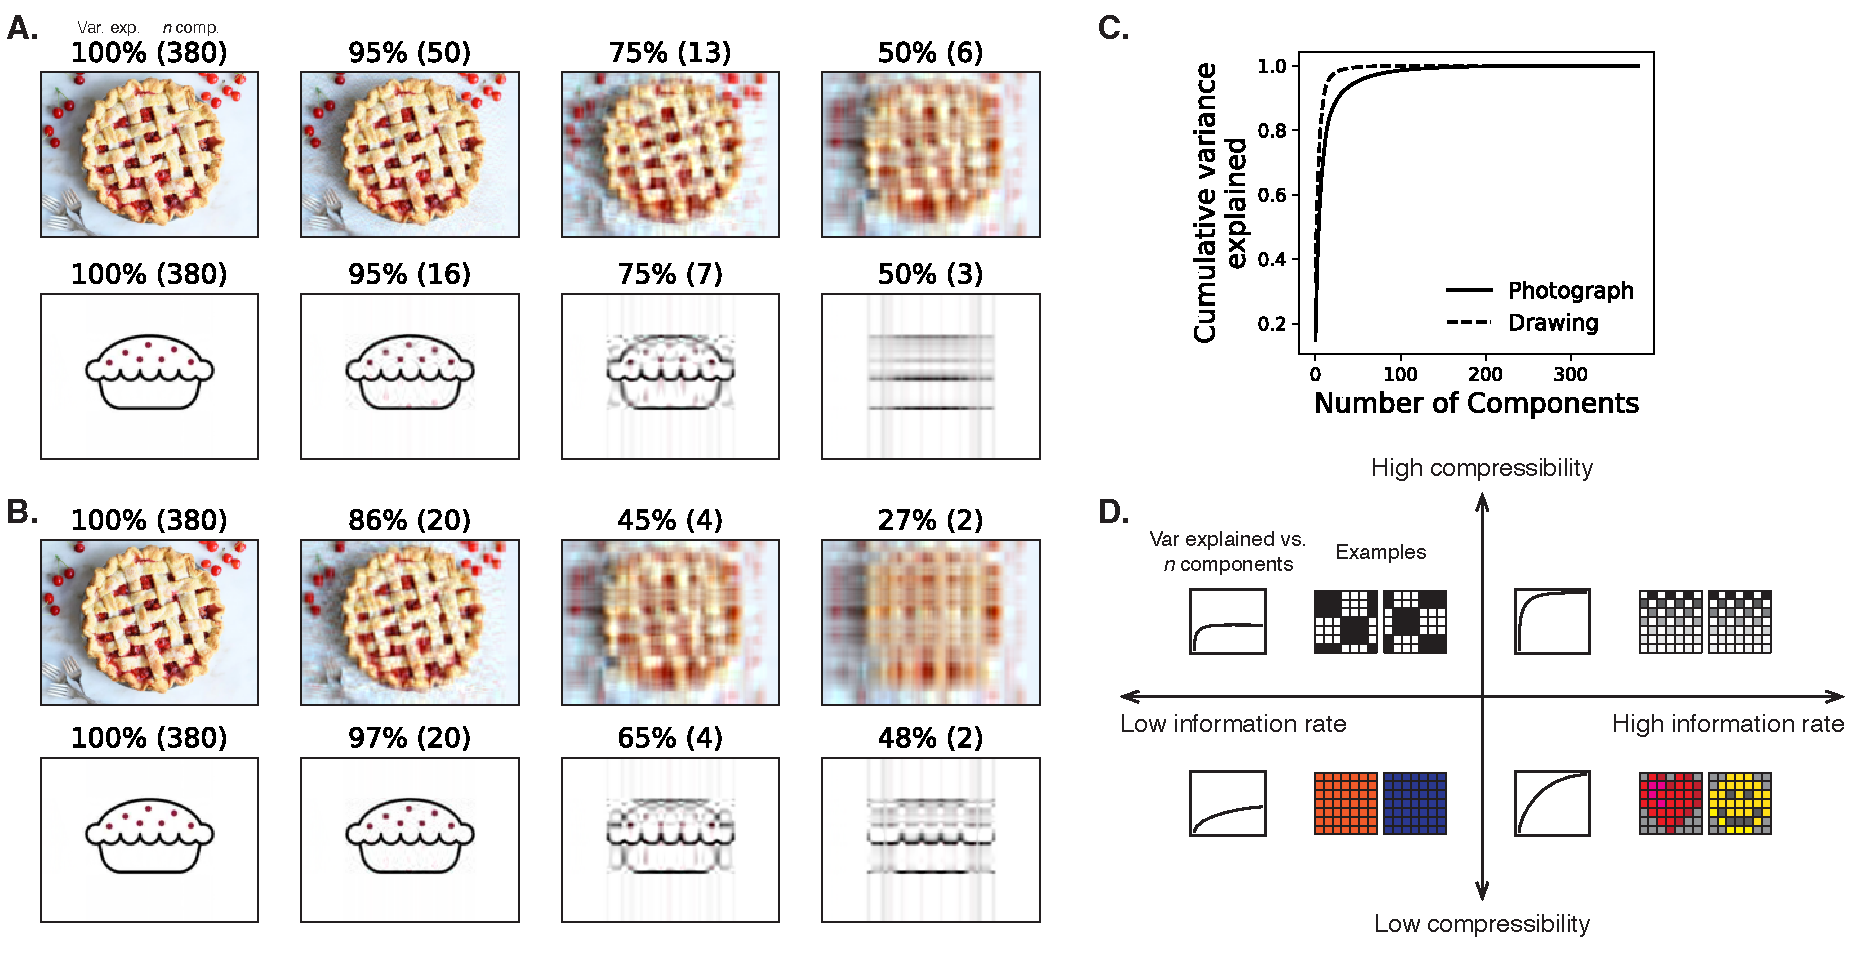
\includegraphics[width=\textwidth]{figs/information_and_compressibility}
  
  \caption{\textbf{Information content and compressibility.} \textbf{A.
  Variance explained for two images.} We applied principal components analysis
  to a photograph and drawing, treating the rows of the images as
  ``observations.'' Across columns, we identified the numbers of components
  required to explain 100\%, 95\%, 75\%, or 50\% of the cumulative variance in
  each image (the 100\% columns denote the original images). The numbers of
  components are indicated in parentheses, and the resulting ``compressed''
  images are displayed. \textbf{B. Representing two images with different
  numbers of components.} Using the same principal component decompositions as
  in Panel A, we computed the cumulative proportion of variance explained with
  380 (original images), 20, 4, or 2 components. \textbf{C. Cumulative variance
  explained versus number of components.} For the images displayed in Panels A
  and B, we plot the cumulative proportion of variance explained as a function
  of the number of components used to represent each image. \textbf{D.
  Information rate and compressibility.} Across multiple images, the
  information rate (i.e., the amount of information contained in each image;
  horizontal axis) is high when each individual pixel provides information that
  cannot be inferred from other pixels. High-information rate images tend to be
  high-resolution, and low-information rate images tend to be low-resolution.
  Compressibility is related to the difference between the information required
  to specify the original versus compressed images (vertical axis). Highly
  compressible images often contain predictable structure (redundancies) that
  can be leveraged to represent the images much more efficiently than in their
  original feature spaces.}

\label{fig:information-compression} 
\end{figure}

To the extent that brain activity patterns contain rich task-relevant
information, we should be able to use the activity patterns to accurately
differentiate between different aspects of a task~\citep[e.g., using pattern
classifiers;][]{NormEtal06b}. For example, prior work has shown a direct
correspondence between classification accuracy and the information content of a
signal~\citep{Alva02}. To the extent that brain activity patterns are
compressible, we should be able to generate simplified (e.g., lower
dimensional) representations of the data while still preserving the relevant or
important aspects of the original signal. In general, information content and
compressibility are related but are partially dissociable
(Fig.~\ref{fig:information-compression}). If a given signal (e.g., a
representation of brain activity patterns) contains more information about
ongoing cognitive processes, then the peak decoding accuracy should be high.
And if the signal is compressible, a low-dimensional embedding of the signal
will be similarly informative as the original signal
(Fig.~\ref{fig:information-compression}D).


Several recent studies suggest that the complexity of brain activity is
task-dependent, whereby simpler tasks with lower cognitive demands are
reflected by simpler and more compressible brain activity patterns, and more
complex tasks with higher cognitive demands are reflected by more complex and
less compressible brain activity patterns~\citep{MackEtal20, OwenEtal21}. These
findings complement other work suggesting that functional connectivity
(correlation) patterns are task-dependent~\citep{FinnEtal17, OwenEtal20,
ColeEtal14}, although see~\cite{GratEtal18}. Higher-order cognitive processing
of a common stimulus also appears to drive more stereotyped task-related
activity and functional connectivity across individuals~\citep{HassEtal08,
LernEtal11, SimoChan20, SimoEtal16}.

The above studies are consistent with two potential descriptions of how
cognitive processes are reflected in brain activity patterns. One possibility
is that the information rate of brain activity increases during more complex or
higher-level cognitive processing. If so, then the ability to reliably decode
cognitive states from brain activity patterns should improve with task
complexity or with the level (or ``depth'') of cognitive processing. A second
possibility is that the compressibility of brain activity patterns increases
during more complex or higher-level cognitive processing. If so, then
individual features of brain recordings, or compressed representations of brain
recordings, should carry more information during complex or high-level (versus
simple or low-level) cognitive tasks.

We used a previously collected neuroimaging dataset to estimate the extent to
which each of these two possibilities might hold. The dataset we examined
comprised functional magnetic resonance imaging (fMRI) data collected as
participants listened to an audio recording of a 10-minute story, temporally
scrambled recordings of the story, or underwent a resting state
scan~\citep{SimoEtal16}. Each of these experimental conditions evokes different
depths of cognitive processing~\citep{SimoEtal16,LernEtal11,
HassEtal08,OwenEtal21}. We used across-participant classifiers to decode
listening times in each condition, as a proxy for how ``informative'' the
task-specific activity patterns were~\citep{SimoChan20}. We also used principle
components analysis to generate lower-dimensional representations of the
activity patterns. We then repeated the classification analyses after
preserving different numbers of components and examined how classification
accuracy changed across the different experimental conditions.



\section*{Results}

We sought to understand whether higher-level cognition is reflected by more
reliable and informative brain activity patterns, and how compressibility of
brain activity patterns relates to cognitive complexity. We developed a
computational framework for systematically assessing the informativeness and
compressibility of brain activity patterns recorded under different cognitive
circumstances. We used across-participant decoding accuracy (see
\textit{Forward inference and decoding accuracy}) as a proxy for
informativeness. To estimate the compressibility of the brain patterns, we used
group principal components analysis (PCA) to project the brain patterns into
$k$-dimensional spaces, for different values of $k$ (see \textit{Hierarchical
Topographic Factor Analysis (HTFA)} and \textit{Principal components analysis
(PCA)}). For more compressible brain patterns, decoding accuracy should be more
robust to small values of $k$.

We analyzed a dataset collected by \cite{SimoEtal16} that comprised four
experimental conditions. These conditions exposed participants to stimuli that
systematically varied in cognitive engagement. In the \textit{intact}
experimental condition, participants listened to an audio recording of a
10-minute Moth Radio Hour story, \textit{Pie Man}, by Jim O'Grady. In the
\textit{paragraph}-scrambled experimental condition, participants listened to a
temporally scrambled version of the story, where the paragraphs occurred out of
order, but where the same set of paragraphs was presented over the entire
listening interval. All participants in this condition experienced the
scrambled paragraphs in the same order. In the \textit{word}-scrambled
experimental condition, participants listened to a temporally scrambled version
of the story, where the words occurred in a random order. Again, all
participants in this condition experienced the scrambled words in the same
order. Finally, in the \textit{rest} experimental condition, participants lay
in the scanner with no overt stimulus, while keeping their eyes open and
blinking as needed. This public dataset provided a convenient means for testing
our hypothesis that different levels of cognitive processing and engagement
affect how informative and compressible the associated brain patterns are.

\begin{figure}[tp]
  \centering
  
  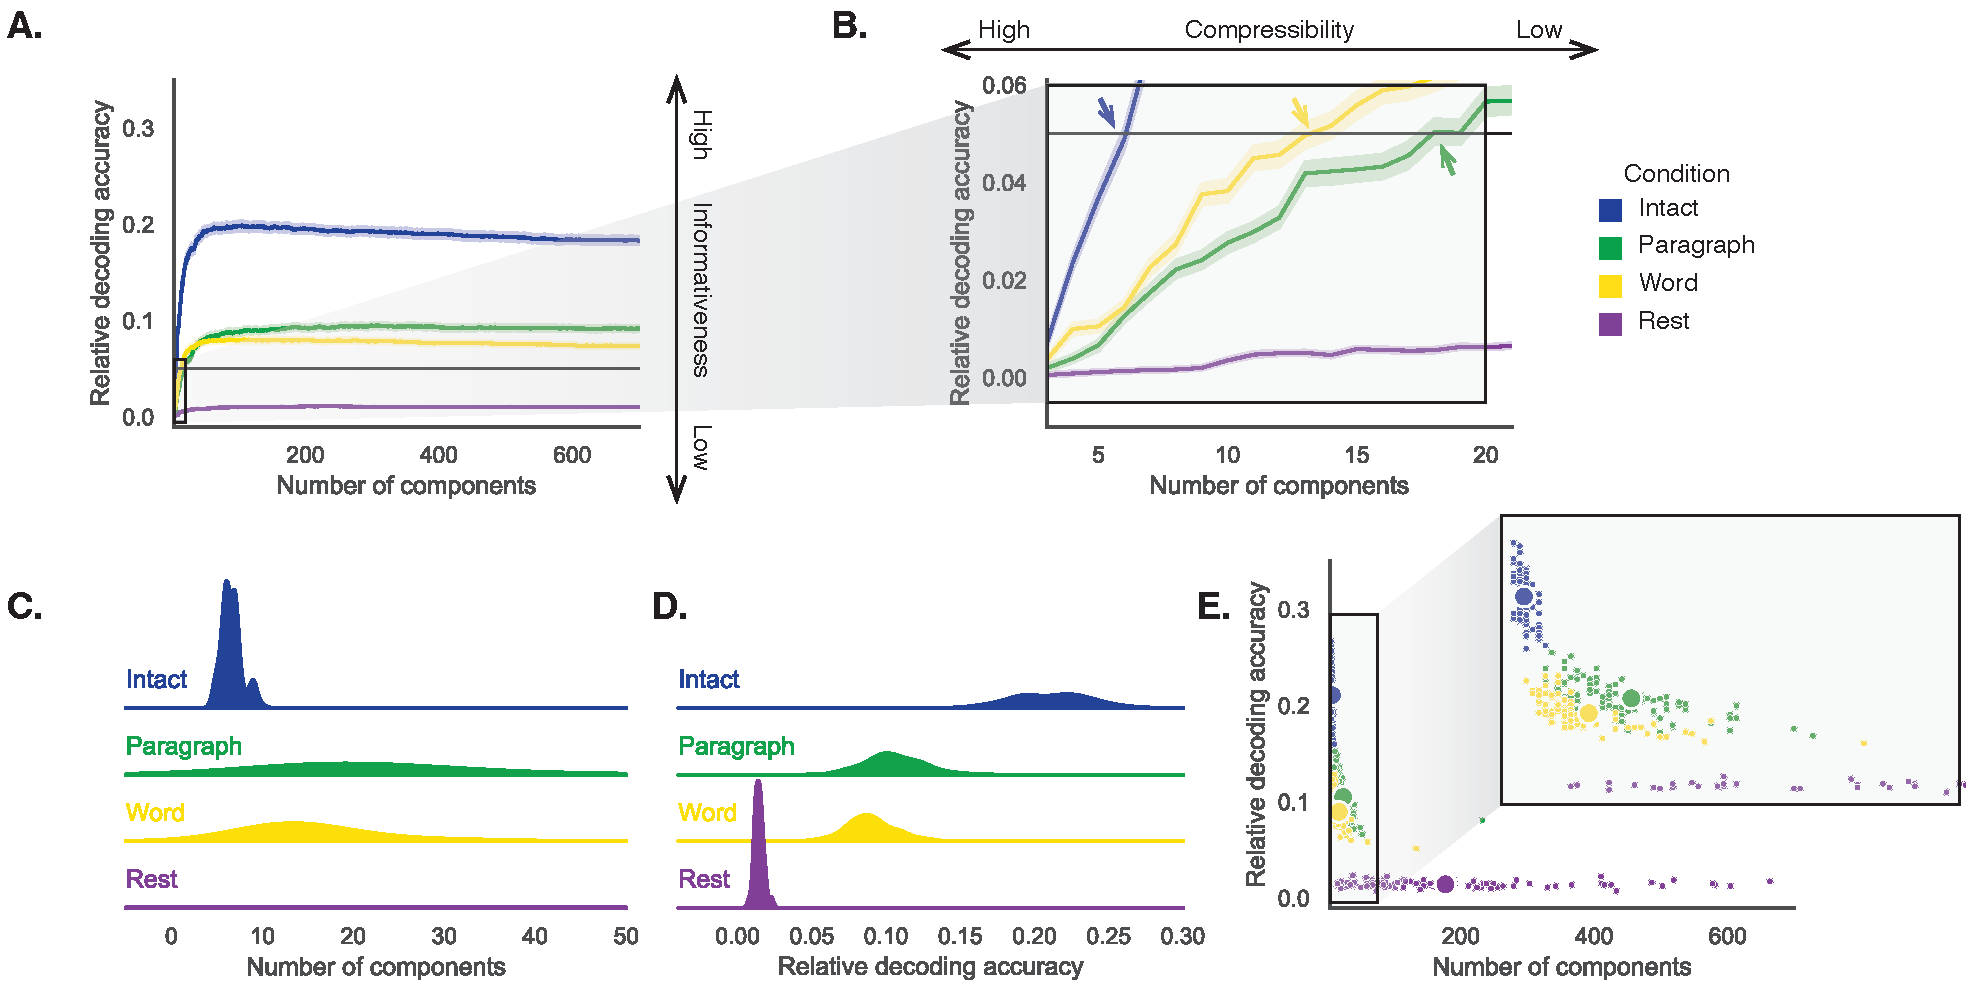
\includegraphics[width=\textwidth]{figs/decoding_and_inflection}

\caption{\textbf{Decoding accuracy and compression.} \textbf{A. Decoding
accuracy by number of components.} Ribbons of each color display
cross-validated decoding performance for each condition (intact, paragraph,
word, and rest), as a function of the number of components (features) used to
represent the data. For each condition, decoding accuracy has been normalized
by subtracting expected ``chance'' decoding performance (estimated as
$\frac{1}{T}$, where $T$ is the number of timepoints in the given condition).
This normalization was intended to enable fairer comparisons across conditions;
a relative decoding accuracy of 0.0 denotes ``chance'' performance. The
horizontal black line denotes 5\% decoding accuracy (used as a reference in
Panel B). \textbf{B. Numbers of components required to reach a fixed decoding
accuracy threshold, by condition.} The panel displays a zoomed-in view of the
inset in Panel A. Intersections between each condition's decoding accuracy
curve and the 5\% decoding accuracy reference line are marked by arrows. All
error ribbons in Panels A and B denote bootstrap-estimated 95\% confidence
intervals. \textbf{C. Estimating ``compressibility'' for each condition.} The
density plots display the numbers of components required to reach at least 5\%
(corrected) decoding accuracy, across all cross validation runs. For the
``rest'' condition, where decoding accuracy never reached 5\% accuracy, we
display the distribution of the numbers of components required to achieve the
peak decoding accuracy in each fold. (This distribution is nearly flat, as
also illustrated in Panel E.) \textbf{D. Estimating ``informativeness'' for each
condition.} The density plots display the peak (corrected) decoding accuracies
achieved in each condition, across all cross validation runs. \textbf{E.
Informativeness versus compressibility.} Each dot displays the minimum number
of components required to achieve at least 5\% corrected decoding accuracy
($x$-coordinate; for the rest condition the numbers of components are estimated
using the peak decoding accuracies as in Panel C) and the peak (corrected)
decoding accuracy ($y$-coordinate). The smaller dots correspond to individual
cross validation runs and the larger dots display the averages across runs. The
inset displays a zoomed-in view of the indicated region in the main panel.}

\label{fig:inflection}
\end{figure}

To evaluate the relation between informativeness and compressibility for brain
activity from each experimental condition, we trained a series of
across-participant temporal decoders on compressed representations of the data.
Figure~\ref{fig:inflection}A displays the decoding accuracy as a function of
the number of principal components used to represent the data (also see
Fig.~\varExplained). Several patterns were revealed by the analysis. First, in
general (i.e., across experimental conditions), decoding accuracy tends to
improve as the number of components are increased. However, decoding accuracy
peaked at higher levels for experimental conditions that exposed participants
to cognitively richer stimuli (Fig.~\ref{fig:inflection}D). The peak decoding
accuracy was highest for the ``intact'' condition (versus paragraph: $t(99) =
35.205, p < 0.001)$; versus word: $t(99) = 43.172, p < 0.001)$; versus rest:
$t(99) = 81.361, p < 0.001)$), next highest for the ``paragraph'' condition
(versus word: $t(99) = 6.243, p < 0.001)$; versus rest: $t(99) = 50.748, p <
0.001)$), and next highest for the ``word'' condition (versus rest: $t(99) =
48.791, p < 0.001)$). This ordering implies that cognitively richer conditions
evoke more stable brain activity patterns across people.

The cognitively richer conditions also displayed steeper initial slopes. For
example, the intact condition decoders reached an arbitrarily chosen threshold
of 5\% accuracy using fewer components than the paragraph condition decoders
($t(99) = -7.429, p < 0.001$) or word condition decoders ($t(99) = -7.300, p <
0.001$), and decoding accuracy never exceeded 5\% for the rest condition. This
suggests that brain activity patterns evoked by cognitively richer conditions
are more compressible, such that representing the data using the same number of
principal components provides more information to the temporal decoders
(Figs.~\ref{fig:inflection}B, C). Taken together, as shown in
Figure~\ref{fig:inflection}E, we found that brain activity patterns evoked by
cognitively richer conditions tended to be both more informative (i.e.,
associated with higher peak decoding accuracies) \textit{and} more compressible
(i.e., requiring fewer components to achieve the 5\% accuracy threshold).


\begin{figure}[tp]
  \centering
  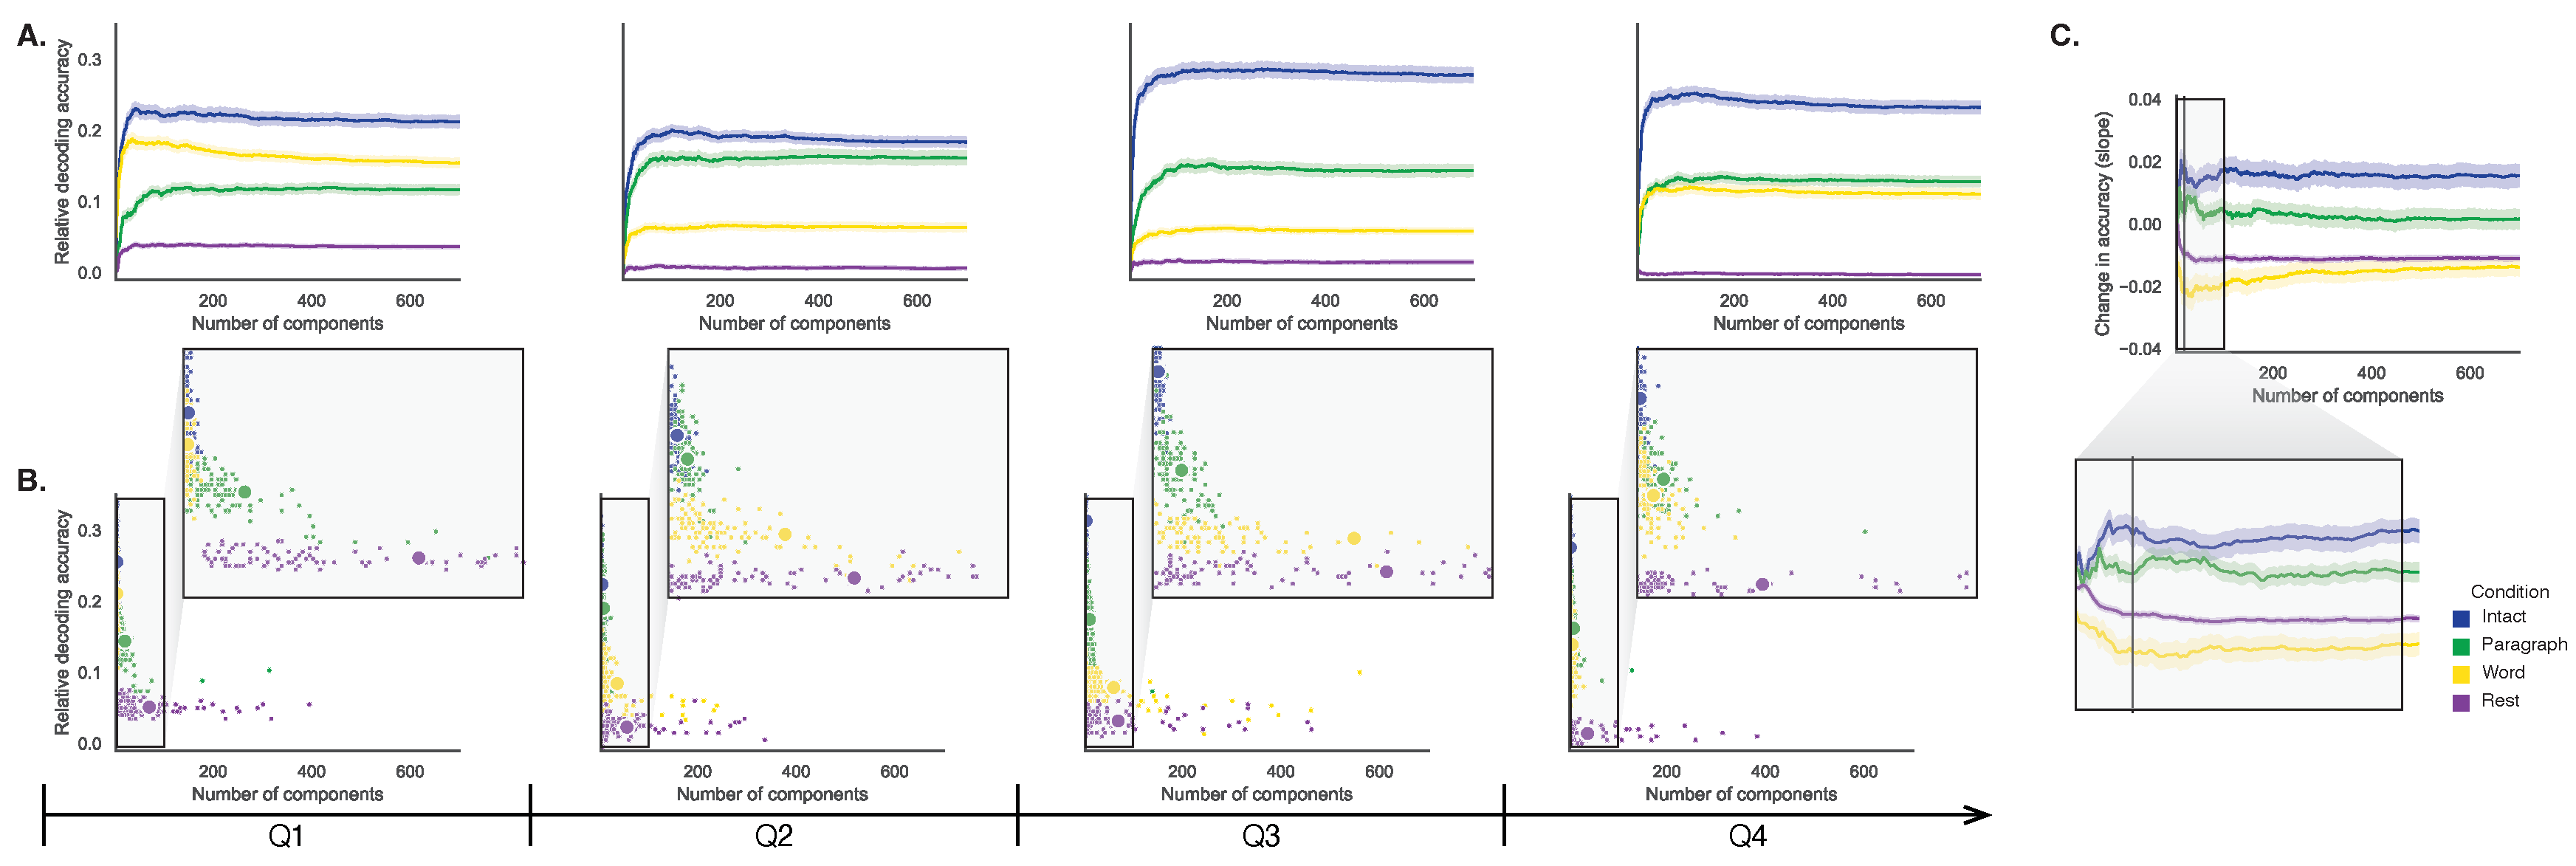
\includegraphics[width=\textwidth]{figs/information_and_compression_over_time}

\caption{\textbf{Changes in decoding accuracy and compression over time.}
\textbf{A. Decoding accuracy by number of components, by story segment.} Each
family of curves is plotted in the same format as Figure~\ref{fig:inflection}A
but reflects data only from one quarter of the dataset. \textbf{B.
Informativeness versus compressibility by condition and segment.} Each scatter
plot is in the same format as Figure~\ref{fig:inflection}E, but reflects data
only from one quarter of the dataset. \textbf{C. Change in decoding accuracy
over time, by number of components.} For each number of components ($x$-axis)
and condition (color), we fit a regression line to the decoding accuracies
obtained for the first, second, third, and fourth quarters of the dataset
(corresponding to the columns of Panels A and B). The $y$-axis denotes the
slopes of the regression lines. The black vertical line marks $k = 20$ components,
as referenced in the main text.  All error ribbons denote bootstrap-estimated
95\% confidence intervals.}

\label{fig:inflection-quarters}

\end{figure}


If informativeness (to the temporal decoders) and compressibility vary with the
cognitive richness of the stimulus, might these measures also vary over time
\textit{within} a given condition? For example, participants in the intact
condition might process the ongoing story more deeply later on in the story
(compared with earlier in the story) given the additional narrative background
and context they had been exposed to by that point. To examine this
possibility, we divided each condition into four successive time segments. We
computed decoding curves (Fig.~\ref{fig:inflection-quarters}A) and the numbers
of components required to achieve 5\% decoding accuracy
(Fig.~\ref{fig:inflection-quarters}B) for each segment and condition. We found
that, in the two most cognitively rich conditions (intact and paragraph), both
decoding accuracy and compressibility, as reflected by the change in decoding
curves, increased with listening time (e.g., at the annotated reference point
of $k = 20$ components in Fig.~\ref{fig:inflection-quarters}C: intact: $t(99) =
7.915, p < 0.001$; paragraph: $t(99) = 2.354, p = 0.021$). These changes may
reflect an increase in comprehension or depth of processing with listening
time. In contrast, the decoding accuracy and compressibility \textit{decreased}
with listening time in the word condition ($t(99) = -10.747, p < 0.001$) and
rest condition ($t(99) = -22.081, p < 0.001$). This might reflect the
depletion of attentional resources in the less-engaging word and rest
conditions.

\begin{figure}[tp]
  \centering
  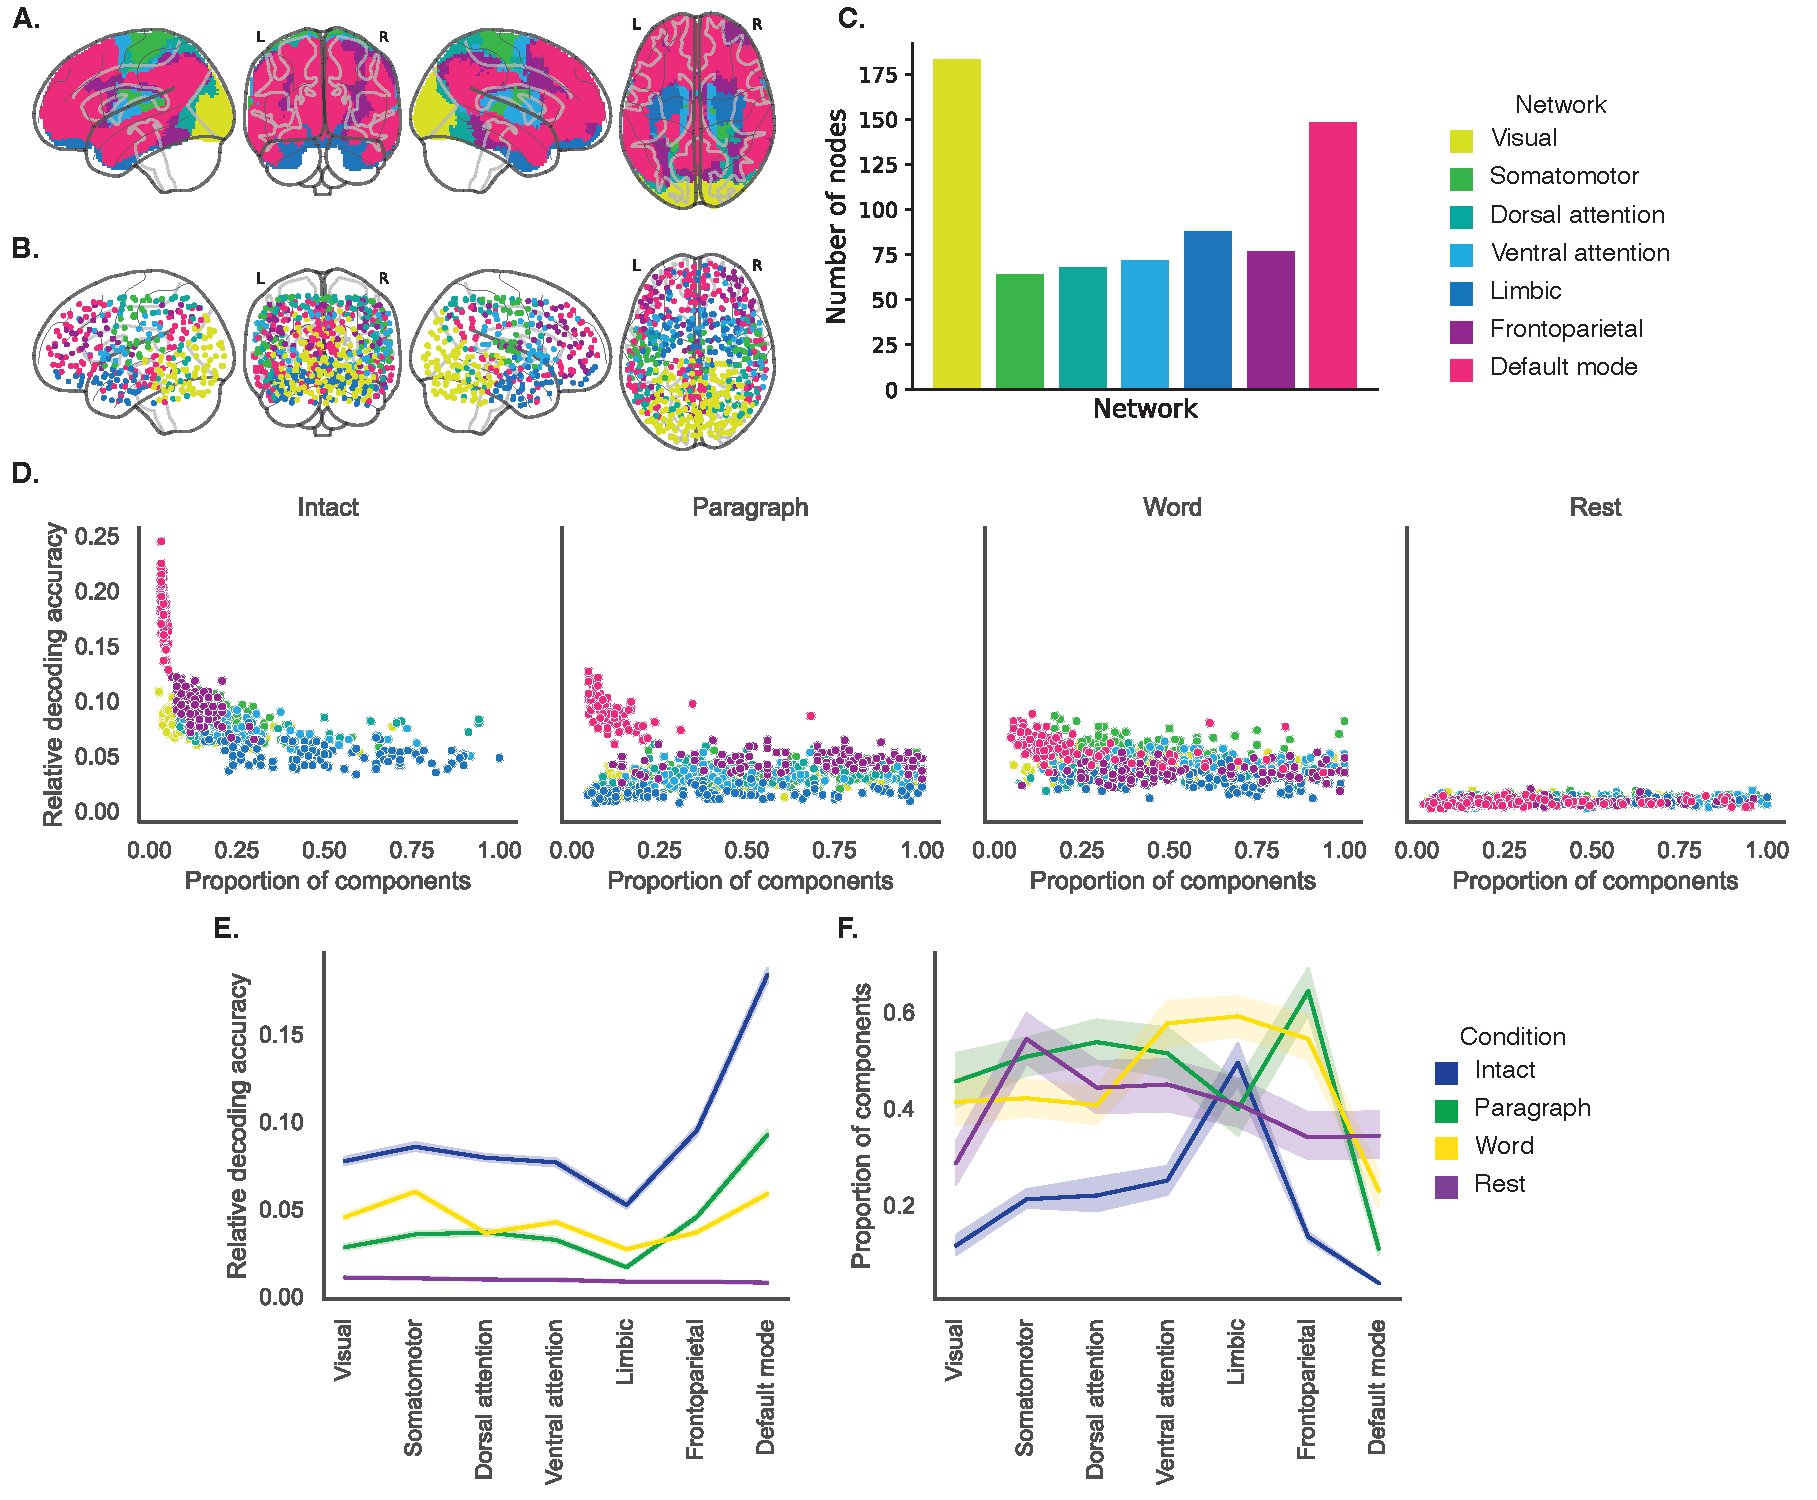
\includegraphics[width=0.9\textwidth]{figs/network_results}

  \caption{\textbf{Network-specific decoding accuracy and compression.}
  \textbf{A. Network parcellation map.} The glass brain displays the location
  of each of seven networks identified by \cite{YeoEtal11}. \textbf{B. Node
  labels.} We assigned network labels to each of 700 Hierarchical Topographic
  Factor Analysis-derived nodes (see \textit{Hierarchical topographic factor
  analysis (HTFA)}). For each node, we evaluated its radial basis function
  (RBF) at the locations of every voxel in the parcellation map displayed in
  Panel A. We summed up these RBF weights separately for the voxels in each
  network. We defined each node's network label as its highest-weighted network
  across all voxels. \textbf{C. Per-network node counts.} The bar plot displays
  the total number of HTFA-derived nodes assigned to each network. \textbf{D.
  Informativeness versus compressibility by network and condition.} Each dot
  corresponds to a single cross validation run. The dots' coordinates denote
  the minimum proportion of components (relative to the number of nodes in the
  given network) required to achieve at least 5\% corrected decoding accuracy
  ($x$-coordinate; for the rest condition these proportions are estimated using
  the peak decoding accuracies) and peak (corrected) decoding accuracy
  ($y$-coordinate). We repeated the analysis separately for each network
  (color) and experimental condition (column). \textbf{E. Informativeness by
  network.} For each network, sorted (roughly) from lower-order networks on the
  left to higher-order networks on the right, the curves display the peak
  (corrected) decoding accuracy for each experimental condition (color).
  \textbf{F. Compressibility by network.} For each network, the curves display
  the proportion of components (relative to the total possible number of
  components displayed in Panel C) required to achieve at least 5\% decoding
  accuracy (or, for the rest condition, peak decoding accuracy, as described
  above). Error ribbons in Panels E and F denote bootstrap-estimated
  95\% confidence intervals.}

  \label{fig:networks}
\end{figure}

We also wondered how informativeness and compressibility in the different
experimental conditions might vary across brain networks. We used a network
parcellation identified by \cite{YeoEtal11} to segment the brain into seven
distinct networks. The networks can be sorted (roughly) in order from
lower-level to higher-level cortex as follows (Figs.~\ref{fig:networks}A--C):
visual, somatomotor, dorsal attention, ventral attention, limbic,
frontoparietal, and default mode. Next, we computed decoding curves separately
for the activity patterns within each network and identified each network's
inflection point, for each experimental condition. Moving from low-order
networks to higher-order networks, we found that decoding accuracy tended to
increase, particularly in the higher-level experimental conditions
(Fig.~\ref{fig:networks}D, E). This suggests that higher-order networks may
carry more content-relevant or stimulus-driven ``information.'' We found no
clear trends in the proportions of components required to achieve 5\% decoding
accuracy across networks or conditions (Fig.~\ref{fig:networks}F).

\begin{figure}[tp]
  \centering
  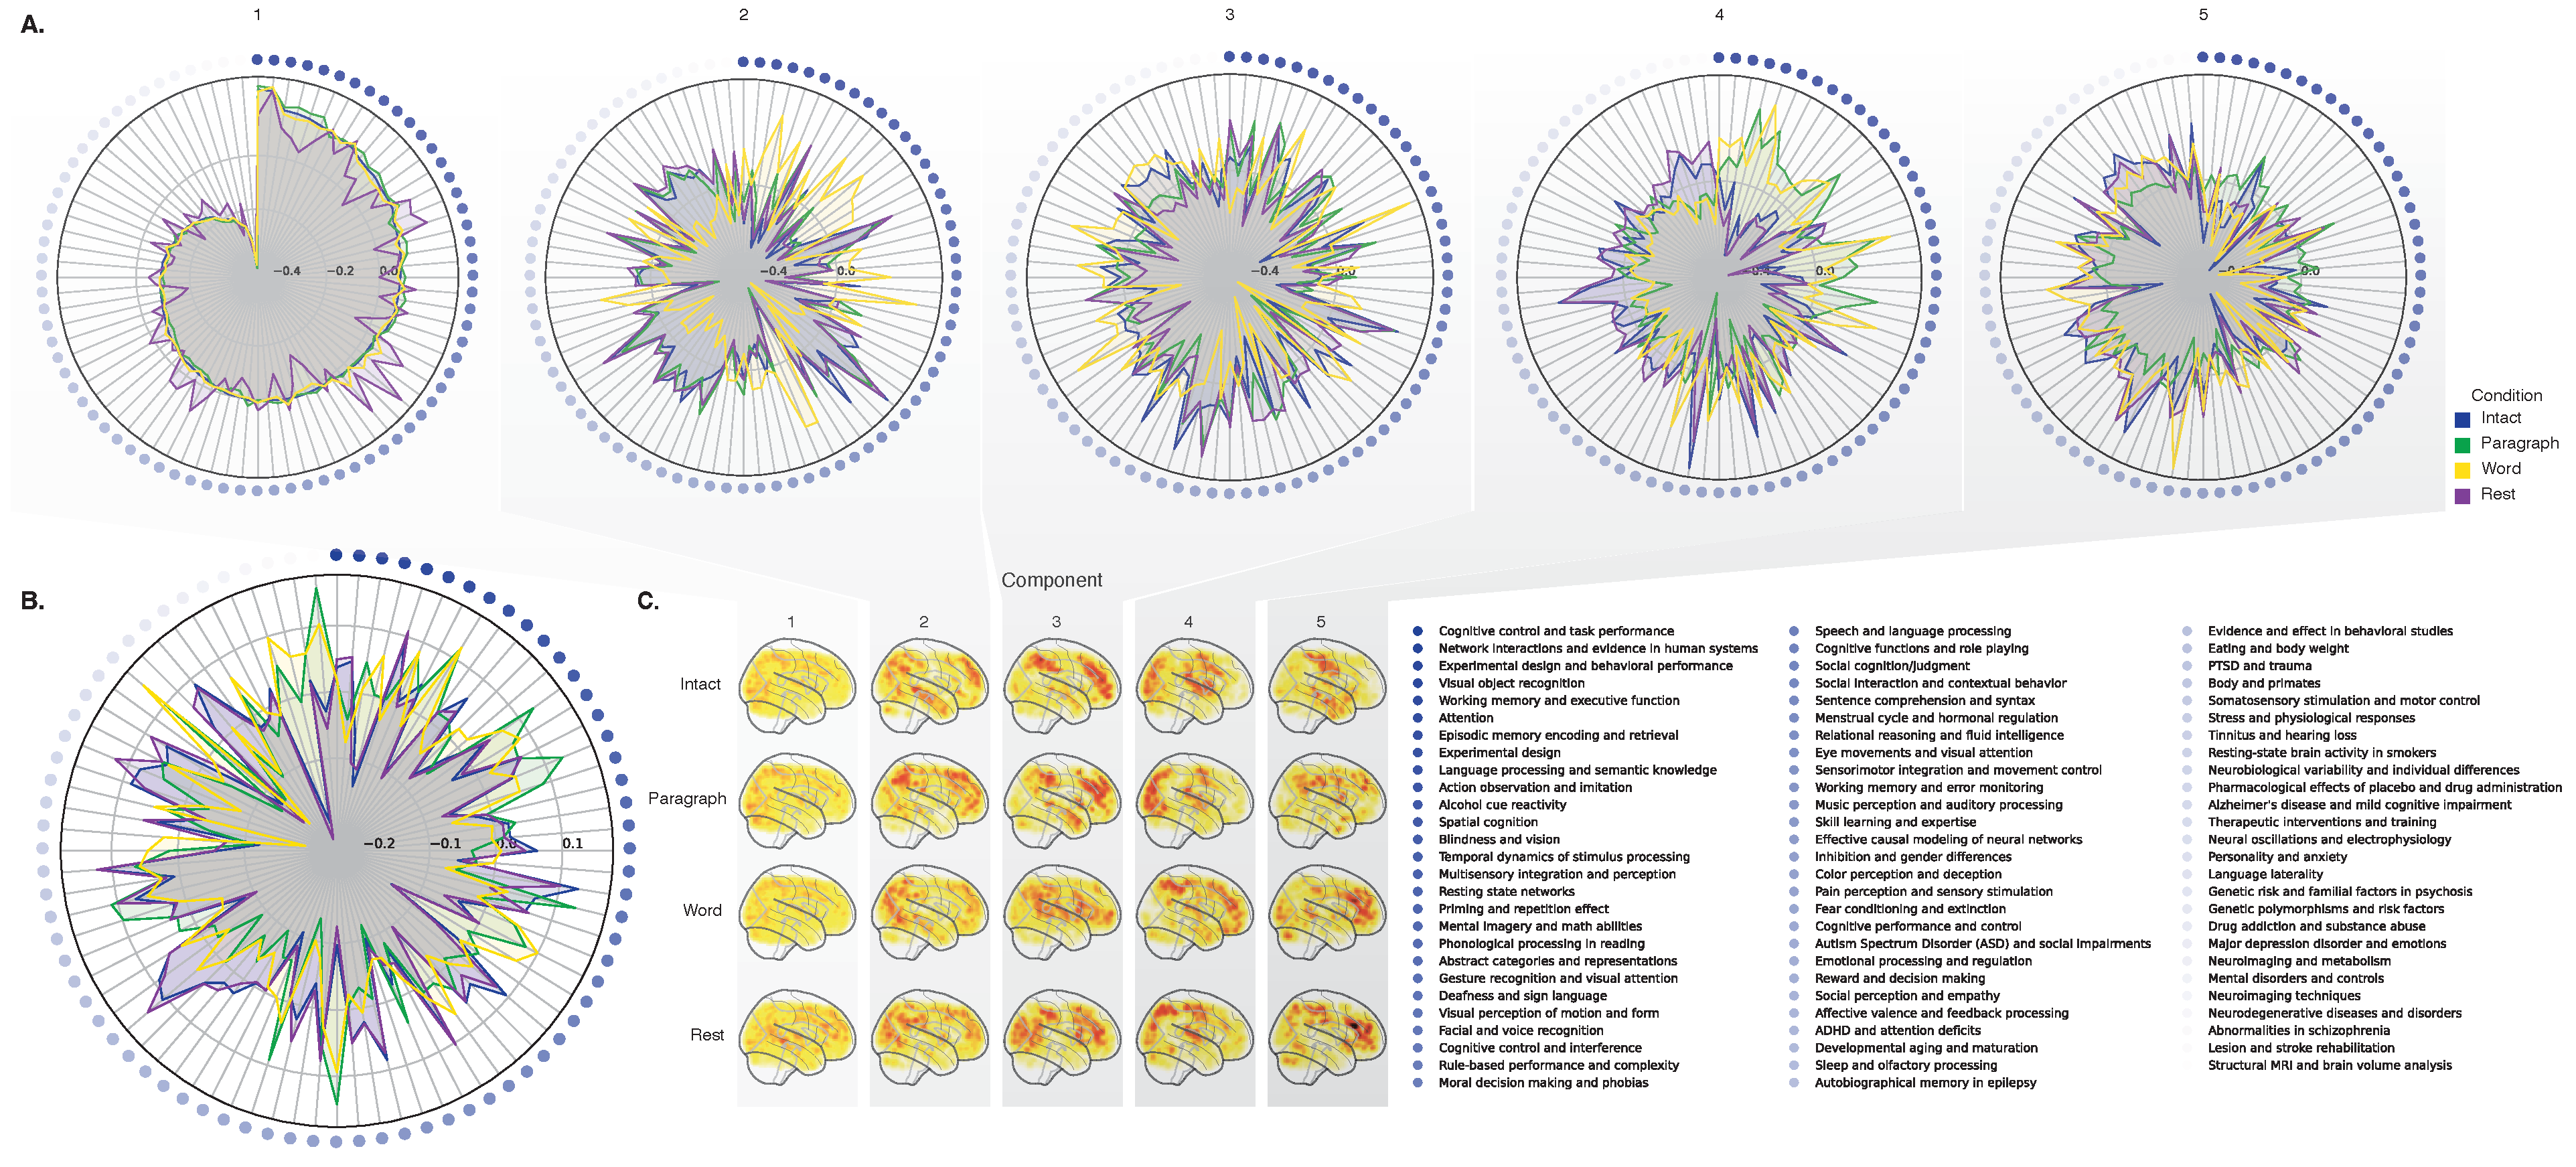
\includegraphics[width=\textwidth]{figs/neurosynth_by_component}

\caption{\textbf{Neurosynth topic weightings by component.} We used a reverse
inference procedure (see \textit{Reverse inference}) to estimate the
correspondences between brain images and a set of 80 topics derived from the
Neurosynth database of neuroimaging articles~\citep{RubiEtal17}. \textbf{A.
Topic correlations by component.} For each of the top five highest-weighted
principal components (columns) derived from each experimental condition
(colors), the radar plots display the correlations between the component images
and the per-topic images derived for each topic (topic identities are denoted
by the blue dots; a legend for the topic labels is in the lower right of the
figure). An annotated list of the top-weighted topics for each component and
condition may be found in Figure~\topTerms~and the top-weighted terms for each
topic may be found in Table~\topics. \textbf{B. Topic correlations averaged
across components.} The radar plot is in the same format as the plots in Panel
A, but here we display the per-condition average correlations across the top
five components (for each condition) reflected in Panel A. \textbf{C. Component
images.} Each plot displays a right sagittal view of a glass brain projection of
the top five principal components (columns) for each experimental condition
(rows). Additional projections for each component may be found in
Figure~\componentBrains.}

\label{fig:neurosynth-pca}

\end{figure}

In addition to examining different networks in isolation, we wondered about the
general structure of the full-brain (i.e., potentially multi-network) activity
patterns reflected by different principal components across different
experimental conditions. As shown in Figure~\ref{fig:neurosynth-pca}, we used
Neurosynth~\citep{RubiEtal17} to identify, for each component, the associations
with each of 80 themes (see \textit{Reverse inference}).  In general, the first
principal components across all of the experimental conditions tended to weight
most heavily on themes related to cognitive control, memory,
language processing, attention, and perception.  Other components appeared to
vary more across conditions.

To gain further insights into which brain functions might be most closely
associated with the top-weighted components from each experimental condition,
we manually grouped each Neurosynth-derived topic into a smaller set of core
cognitive functions. Separately for each component, we computed the average
weightings across all topics that were tagged as being associated with each of
these cognitive functions (Figs.~\ref{fig:neurosynth-summary}A,~\neurosynthFull
A). To help visualize these associations, we used the patterns of associations
for each component to construct graphs whose nodes were experimental conditions
and cognitive functions (Figs.~\ref{fig:neurosynth-summary}B,~\neurosynthFull
B). We also computed correlations between the sets of per-topic weightings from
each of the top-weighted components from each experimental condition
(Fig.~\ref{fig:neurosynth-summary}C, D) and between the brain maps for each
condition's components (Fig.~\neurosynthFull C, D). Taken together, we found
that each component appeared to weight on a fundamental set of cognitive
functions that varied by experimental condition. For example, the top principal
components from every condition weighted similarly (across conditions) on the
full set of Neurosynth topics (Fig.~\ref{fig:neurosynth-pca}A) and cognitive
functions (Figs.~\ref{fig:neurosynth-summary}A, B and~\neurosynthFull~A, B),
suggesting that these components might reflect a set of functions or activity
patterns that are common across all conditions. The second components'
weightings were similar across the intact, paragraph, and rest conditions
(highest-weighted functions: cognitive control, memory, social cognition, and
resting state), but different for the word condition (highest-weighted
functions: sensory perception and cognitive control). The fourth components'
weighting grouped the paragraph and word conditions (highest-weighted
functions: memory, language processing, and cognitive control) and the intact
and rest conditions (highest-weighted functions: emotion, social cognition). We
also used ChatGPT~\citep{ChatGPT} to sort the list of manually tagged cognitive
functions from lowest-level to highest-level (Tab.~\topicTags,
Fig.~\ref{fig:neurosynth-summary}E; also see \textit{Ranking cognitive
processes}). We found that higher-level functions tended to be weighted on more
heavily by top components from the intact and paragraph conditions than
lower-level functions. The top components from the word condition showed the
opposite tendency, whereby \textit{lower}-level functions tended to be weighted
on more heavily than higher-level functions. The components from the rest
condition showed almost no differences in the weights associated with
high-level versus low-level functions.

\begin{figure}[tp]
  \centering
  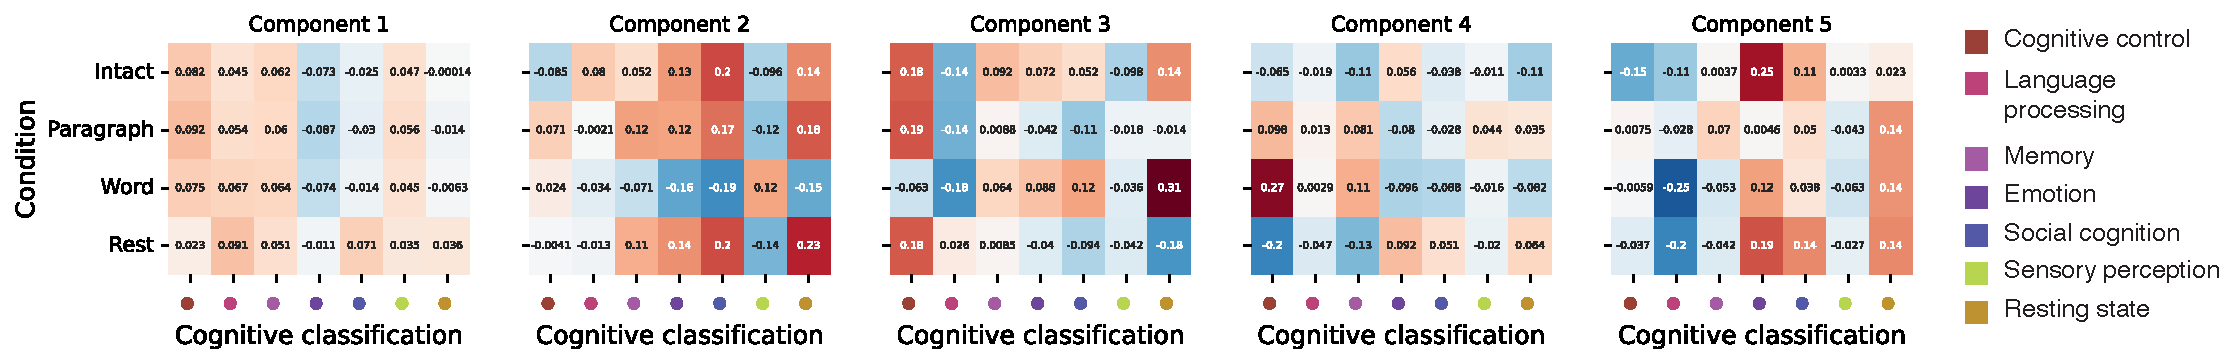
\includegraphics[width=0.9\textwidth]{figs/components_neurosynth_summary}

\caption{\textbf{Summary of functions associated with top-weighted components
by condition.} \textbf{A. Top-weighted topics by condition.} Here we display
per-condition (rows, indicated by colored dots) topic correlations, averaged
across topics that pertain to each of several broad cognitive functions
(columns within each sub-panel, indicated by colored dots). Each sub-panel
reflects correlations for the components indicated in the panel titles. A
legend for the condition and several core cognitive function classifications is
displayed in the lower right of the figure. Table~\topics~provides a list of
each topic's top-weighted terms, along with each topic's manually labeled
cognitive classification. A full list of the topics most highly associated with
each component may be found in Figure~\topTerms. \textbf{B. Associations
between per-condition components and cognitive functions.} The network plots
denote positive average correlations between the component images for each
condition (gray-outlined dots on the left sides of each network; colors denote
conditions) and topic-specific brain maps associated with each indicated
cognitive function (black-outlined dots on the right sides of each network;
colors denote cognitive functions). The line thicknesses are proportional to
the correlation values (correlation coefficients are noted in the heat maps in
Panel A). \textbf{C. Correlations between each principal component, by
condition.} The heat maps display the correlations between the brain maps
(Fig.~\componentBrains) for each principal component (sub-panel), across each
pair of conditions (rows and columns of each sub-panel's matrix, indicated by
colored dots). \textbf{D. Associations between per-condition components, by
component.} Each sub-panel's network plot summarizes the pattern of correlations
between the $n$\textsuperscript{th} top-weighted principal components
(sub-panel) for each experimental condition (gray-outlined dots). The line
thicknesses are proportional to the correlation values (correlation
coefficients are noted in the heat maps in Panel C). \textbf{E. Change in
weights by condition.} The bar heights reflect the slopes of regression lines,
fit separately to the top five components from each condition, between the
ChatGPT-derived ``rank'' of each cognitive classification and the correlations
between the component and topic maps associated with cognitive processes at the
given rank (see \textit{Ranking cognitive processes}).  Also see
Fig.~\neurosynthFull~for additional information.}

\label{fig:neurosynth-summary}
\end{figure}


\section*{Discussion}

We examined fMRI data collected as participants listened to an auditory
recording of a story, scrambled recordings of the story, or underwent a resting
state scan. We found that cognitively richer stimuli evoked more reliable
(i.e., consistent across people) and information rich brain activity patterns.
The brain patterns evoked by cognitively richer stimuli were also more
compressible, in that each individual component provided more ``signal'' to
temporal decoders relative to components of data from less cognitively rich
conditions (Fig.~\ref{fig:inflection}). Over time (e.g., as the experiment
progressed), these phenomena were strengthened. Specifically, across story
segments, data from more cognitively rich conditions became more informative
and compressible, and data from less cognitively rich conditions became
\textit{less} informative and compressible
(Fig.~\ref{fig:inflection-quarters}). We also repeated these analyses
separately for different brain networks. We found that networks traditionally
associated with higher-level cognitive functions tended to provide more
informative brain patterns than networks traditionally associated with lower
level cognitive functions (Fig.~\ref{fig:networks}). Finally, we examined the
most dominant components of the brain activity patterns from each experimental
condition. We used a reverse inference approach~\citep{RubiEtal17} to identify
the terms in the neuroimaging literature most commonly associated with the
corresponding maps. As summarized in Figure~\ref{fig:neurosynth-summary}E, we
found that the intact and paragraph conditions tended to weight on higher-level
cognitive processes more than lower-level cognitive processes, whereas the word
condition weighted on lower-level processes more than higher-level processes
and the rest condition showed no difference in high-level versus low-level
weighting. Taken together, our findings indicate that the informativeness and
compressibility of our brain activity patterns are task-dependent, and these
properties change systematically with factors like cognitive richness and depth
of processing.



Our explorations of informativeness and compressibility are related to a much
broader literature on the correlational and causal structure of brain activity
patterns and networks~\citep{PretEtal17, OwenEtal21, RogeEtal07, RubiSpor10,
SizeEtal18, SmitEtal13b, SmitEtal13c, SrinEtal07, TomaVolk11, YeoEtal11,
AdacEtal12, BassSpor17, BullSpor09, SporHone06, SporBetz16, SporZwi04,
DhamEtal08, KorzEtal08, BrovEtal04, LynnBass21}. Correlations or causal
associations between different brain regions simultaneously imply that
full-brain activity patterns will be compressible and also that those activity
patterns will contain redundancies. For example, the extent to which activity
patterns at one brain area can be inferred or predicted from activity patterns
at other areas~\citep[e.g.,][]{OwenEtal20, ScanEtal21}, reflects overlap in the
information available in or represented by those brain areas. If brain patterns
in one area are recoverable using brain patterns in another area, then a
``signal'' used to convey the activity patterns could be compressed by removing
the recoverable activity. Predictable (and therefore redundant) brain activity
patterns are also more robust to signal corruption. For example, even if the
activity patterns at one region are unreadable or unreliable at a given moment,
that unreliability could be compensated for by other regions' activity patterns
that were predictive of the unreliable region.

Our findings that informativeness and compressibility change with task demands
may follow from task-dependent changes in full-brain correlation patterns. A
number of prior studies have found that so-called ``functional connectivity''
(i.e., correlational) patterns vary reliably across tasks, events, and
situations~\citep{SimoEtal16, ColeEtal14, SmitEtal09, OwenEtal21}. By examining
how these task-dependent changes in correlations affect informativeness and
compressibility, our work suggests a potential reason why the statistical
structure of brain activity patterns might vary with cognitive task or with
cognitive demands. For lower-level tasks, or for tasks that require relatively
little ``deep'' cognitive processing, our brains may optimize activity patterns
for robustness and redundancy over expressiveness, for example to maximize
reliability. For higher-level tasks, or for tasks that require deeper cognitive
processing, our brains may sacrifice some redundancy in favor of greater
expressiveness.

In the information theory sense~\citep{Shan48}, when a signal is transmitted
using a fixed alphabet of ``symbols,'' the information rate decreases as the
signal is compressed (e.g., fewer symbols transmitted per unit time, using an
alphabet with fewer symbols, etc.). Our finding that each individual brain
component (symbol) becomes more informative as cognitive richness increases
suggests that the ``alphabet'' of brain activity patterns is also
task-dependent. Other work suggests that the representations that are
\textit{reflected} by brain activity patterns may also change with task
demands. For example, our brains may represent the same perceptual stimulus
differently depending on which aspects of the stimulus or which combinations of
features are task-relevant~\citep{MackEtal20}.

Different brain networks also varied in how informative and compressible their
activity patterns were across experimental conditions (e.g.,
Fig.~\ref{fig:networks}). This might follow from evolutionary optimizations
that reflect the relevant constraints or demands placed on those networks. One
possibility is that cortex is organized in a hierarchy of networks ``concerned
with'' or selective to different levels of processing or function. To the
extent that different levels of processing (e.g., low-level sensory processing
versus ``deeper'' higher-level processing) reflect different stimulus
timescales~\citep[e.g.,][]{Mann20}, the network differences we observed might
also relate to the timescales at which each network is maximally
sensitive~\citep{RegeEtal18, BaldEtal17,LernEtal11, HassEtal08}.

\subsection*{Concluding remarks}

Cognitive neuroscientists are still grappling with basic questions about the
fundamental ``rules'' describing how our brains respond, and about how brain
activity patterns and the associated underlying cognitive representations and
computations are linked. We identified two aspects of brain activity patterns,
informativeness and compressibility, that appear to change systematically with
task demands and across brain networks. Our work helps to clarify how the
``neural code'' might be structured, and how the code might vary across tasks
and brain areas.

\section*{Methods}

We measured properties of recorded neuroimaging data under different task
conditions that varied systematically in cognitive engagement and depth of
processing. We were especially interested in how \textit{informative} and
\textit{compressible} the activity patterns were under these different
conditions (Fig.~\ref{fig:information-compression}).


\subsection*{Functional neuroimaging data collected during story
  listening}

We examined an fMRI dataset collected by \cite{SimoEtal16} that the authors
have made publicly available at
\href{http://arks.princeton.edu/ark:/88435/dsp015d86p269k}{arks.princeton.edu/ark:/88435/dsp015d86p269k}.
The dataset comprises neuroimaging data collected as participants listened to
an audio recording of a story (intact condition; 36 participants), listened to
temporally scrambled recordings of the same story (17 participants in the
paragraph-scrambled condition listened to the paragraphs in a randomized order
and 36 in the word-scrambled condition listened to the words in a randomized
order), or lay resting with their eyes open in the scanner (rest condition; 36
participants). Full neuroimaging details may be found in the original paper for
which the data were collected~\citep{SimoEtal16}. Procedures were approved by
the Princeton University Committee on Activities Involving Human Subjects, and
by the Western Institutional Review Board (Puyallup, WA). All subjects were
native English speakers with normal hearing and provided written informed
consent.

\subsection*{Hierarchical topographic factor analysis (HTFA)}

Following our prior related work, we used HTFA~\citep{MannEtal18} to derive a
compact representation of the neuroimaging data. In brief, this approach
approximates the timeseries of voxel activations (44,415 voxels) using a much
smaller number of radial basis function (RBF) nodes~\citep[in this case, 700
nodes, as determined by an optimization procedure;][]{MannEtal18}. This
provides a convenient representation for examining full-brain activity patterns
and network dynamics. All of the analyses we carried out on the neuroimaging
dataset were performed in this lower-dimensional space. In other words, each
participant's data matrix was a number-of-timepoints ($T$) by 700 matrix of
HTFA-derived factor weights (where the row and column labels were matched
across participants). Code for carrying out HTFA on fMRI data may be found as
part of the BrainIAK toolbox~\citep{CapoEtal17, KumaEtal21}, which may be
downloaded at \href{https://brainiak.org/}{brainiak.org}.

\subsection*{Principal components analysis (PCA)}

We applied group PCA~\citep{SmitEtal14} separately to the HTFA-derived
representations of the data (i.e., factor loadings) from each experimental
condition. Specifically, for each condition, we considered the set of all
participants' $T$ by 700 factor weight matrices. We used group PCA to project
these 700-dimensional matrices into a series of shared $k$-dimensional spaces,
for $k \in \{3, 4, 5, ..., 700\}$. This yielded a set of number-of-participants
matrices, each with $T$ rows and $k$ columns.

\subsection*{Temporal decoding}

We sought to identify neural patterns that reflected participants' ongoing
cognitive processing of incoming stimulus information. As reviewed by
\cite{SimoEtal16}, one way of homing in on these stimulus-driven neural
patterns is to compare activity patterns across individuals. In particular,
neural patterns will be similar across individuals to the extent that the
neural patterns under consideration are stimulus-driven, and to the extent that
the corresponding cognitive representations are reflected in similar spatial
patterns across people~\citep{SimoChan20}. Following this logic, we used an
across-participant temporal decoding test developed by \cite{MannEtal18} to
assess the degree to which different neural patterns reflected ongoing
stimulus-driven cognitive processing across people. The approach entails using
a subset of the data to train a classifier to decode stimulus timepoints (i.e.,
moments in the story participants listened to) from neural patterns. We use
decoding (forward inference) accuracy on held-out data, from held-out
participants, as a proxy for the extent to which the inputted neural patterns
reflected stimulus-driven cognitive processing in a similar way across
individuals.

\subsubsection*{Forward inference and decoding accuracy}

We used an across-participant correlation-based classifier to decode which
stimulus timepoint matched each timepoint's neural pattern. For a given value
of $k$ (i.e., number of principal components), we first used group PCA to
project the data from each condition into a shared $k$-dimensional space. Next,
we divided the participants into two groups: a template group,
$\mathcal{G}_{\mathrm{template}}$ (i.e., training data), and a to-be-decoded
group, $\mathcal{G}_{\mathrm{decode}}$ (i.e., test data). We averaged the
projected data within each group to obtain a single $T$ by $k$ matrix for each
group. Next, we correlated the rows of the two averaged matrices to form a $T$
by $T$ decoding matrix, $\mathbf{\Lambda}$. In this way, the rows of
$\mathbf{\Lambda}$ reflected timepoints from the template group, while the
columns reflected timepoints from the to-be-decoded group. We used
$\mathbf{\Lambda}$ to assign temporal labels to each timepoint (row) from the
test group's matrix, using the row of the training group's matrix with which it
was most highly correlated. We repeated this decoding procedure, but using
$\mathcal{G}_{\mathrm{decode}}$ as the template group and
$\mathcal{G}_{\mathrm{template}}$ as the to-be-decoded group. Given the true
timepoint labels (for each group), we defined the decoding accuracy as the
average proportion of correctly decoded timepoints, across both groups (where
chance perfomance is $\frac{1}{T}$). In Figures~\ref{fig:inflection}
and~\ref{fig:inflection-quarters} we report the decoding accuracy for each
condition and value of $k$, averaged across $n = 100$ cross validation folds.

\subsection*{Reverse inference}

To help interpret the brain activity patterns we found within the contexts of
other studies, we created summary maps of each principal component, for each
experimental condition. Each principal component comprises 700 ``weights'' on
each of the HTFA-derived RBF nodes (see \textit{Hierarchical Topographic Factor
Analysis}). For each node, we evaluated its RBF at the locations of every voxel
in the standard 2~mm MNI152 template brain and multiplied the RBF by the node's
weight. The sum of these weighted RBF activation maps provides a full-brain
image, in MNI152 space, of the given principal component (Fig.~\componentBrains).

Next, we considered 80 topics estimated using Latent Dirichlet
Allocation~\citep{BleiEtal03} applied to 9,204 functional neuroimaging articles
in the Neurosynth database~\citep{RubiEtal17}. The topics, as well as
associated brain maps identified using Neurosynth, were identified and reported
in several prior studies~\citep{FoxEtal14, SulEtal17, ChenEtal20}. The topic
labels for each topic were generated automatically with the following
ChatGPT~\citep{ChatGPT} prompt: ``Please help me come up with intuitive labels
for topics I found by fitting a topic model to thousands of neuroscience and
psychology articles. I'll paste in the top 10 highest-weighted words for each
topic, and I'd like you to respond with a suggested label. For each topic,
please respond with just the topic label and no other formatting or text. Here
are the next topic's top words:'' followed by a comma-separated list of the
given topic's top-weighted words reflected in the Table~\topics. For some
topics, ChatGPT responded with a longer-form response rather than a concise
topic label. In these instances, on a case-by-case basis, we used a second
follow-up prompt to achieve the given topic's label: ``Could you please come up
with a more concise label for that topic?''. We then manually identified a set
of 11 cognitive labels that were intended to encapsulate a representative range
of widely studied low-level and high-level cognitive functions. In choosing the
set of cognitive labels, we jointly considered each topic's ChatGPT-derived
topic label, along with the top-weighted words for the topic. We attempted to
generate a concise set of labels that still spanned the full set of cognitive
functions reflected across the 80 topics. Topics that appeared unrelated to
specific cognitive functions (e.g., topics related to specific methods or
clinical themes) are designated with dashes in Table~\topics.

Finally, following an approach used in several prior studies~\citep{FoxEtal14,
SulEtal17, ChenEtal20} we treated the correlation between a given component's
brain map and each topic's brain map as an approximate measure of how much the
component was reflective of the given topic. This resulted in a set of 80
``weights'' (correlation coefficients) for each component's brain map, with one
weight per Neurosynth-derived topic.

\subsection*{Ranking cognitive processes}

We manually identified 11 cognitive labels
spanning the set of 80 Neurosynth-derived topics: cognitive control, language
processing, memory, emotion, social cognition, spatial cognition, attention,
reward, sensory perception, motor control, and resting state. We then used
ChatGPT to automatically ``rank'' the processes from high-level to low-level
using the following prompt: ``Please rank these cognitive processes from
highest-level to lowest-level, where higher values indicate higher-order or
higher-level processes. Return the result as a csv file with a header row and
two columns: `Cognitive label' and `Rank'. Here are the processes: cognitive
control, language processing, memory, emotion, social cognition, spatial
cognition, attention, reward, sensory perception, motor control, resting
state''.  Table~\topicTags~displays the output.  We used these labels in
the analysis presented in Figure~\ref{fig:neurosynth-summary}E to help summarize
difference in topic weightings across experimental conditions.





\section*{Data and code availability}

All of the code used to produce the figures and results in this manuscript,
along with links to the corresponding data, may be found at
\href{https://github.com/ContextLab/pca_paper}{github.com/ContextLab/pca\_paper}.

\section*{Acknowledgements} 

We acknowledge discussions with Rick Betzel, Luke Chang, Emily Finn, and Jim
Haxby. Our work was supported in part by NSF CAREER Award Number 2145172 to
J.R.M. The content is solely the responsibility of the authors and does not
necessarily represent the official views of our supporting organizations. The
funders had no role in study design, data collection and analysis, decision to
publish, or preparation of the manuscript.


\section*{Author contributions} 

Conceptualization: J.R.M. and L.L.W.O. Methodology: J.R.M. and L.L.W.O.
Implementation: J.R.M. and L.L.W.O. Analysis: J.R.M. and L.L.W.O. Writing,
Reviewing, and Editing: J.R.M. and L.L.W.O. Funding acquisition: J.R.M.
Supervision: J.R.M.

\bibliographystyle{apacite}
\bibliography{CDL-bibliography/cdl}

\end{document}


